% Chapter 3

\chapter{Study of Wu et. al.'s algorithm for locally optimal NAMO in unknown environments} % Main chapter title

\label{Chapter3} % For referencing the chapter elsewhere, use \ref{Chapter3}

\section{Original algorithms}

\begin{figure}[H]
\centering
\begin{subfigure}{.5\textwidth}
  \centering
  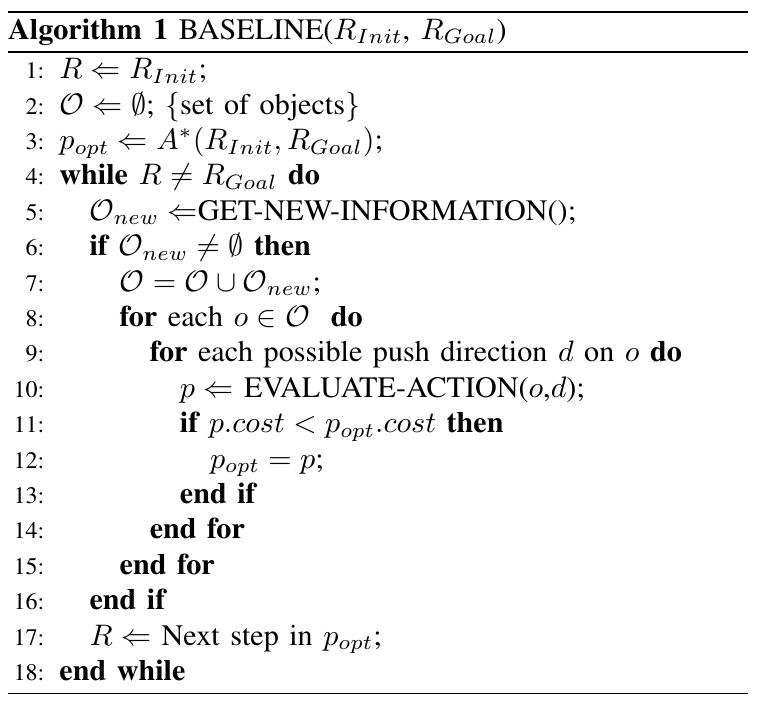
\includegraphics[width=\linewidth]{Figures/Wu_Original_Algorithm/algo1.png}
  \caption{Main loop that evaluates all plans containing the manipulation of an obstacle every time a new one is found}
  \label{fig:Wu_Original_Algorithm-algo1}
\end{subfigure}%
\begin{subfigure}{.5\textwidth}
  \centering
  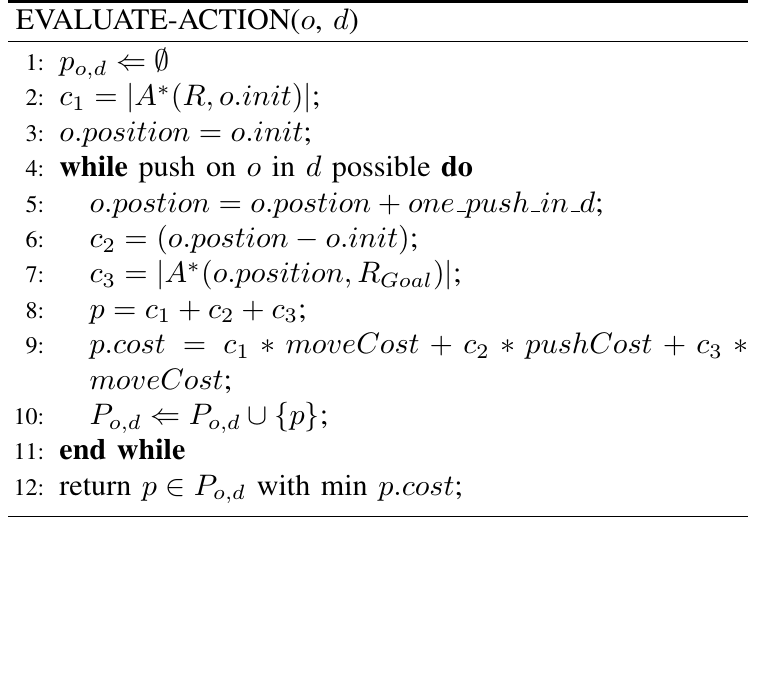
\includegraphics[width=\linewidth]{Figures/Wu_Original_Algorithm/algo2.png}
  \caption{Subroutine for evaluating all possible plans for each manipulation direction allowed on an obstacle}
  \label{fig:Wu_Original_Algorithm-algo2}
\end{subfigure}
\caption{Baseline Algorithm as published by Wu et. al. in \parencite{wu_navigation_2010}}
\label{fig:Wu_Original_Algorithm-baseline}
\end{figure}

\begin{figure}[H]
\centering
\begin{subfigure}{.5\textwidth}
  \centering
  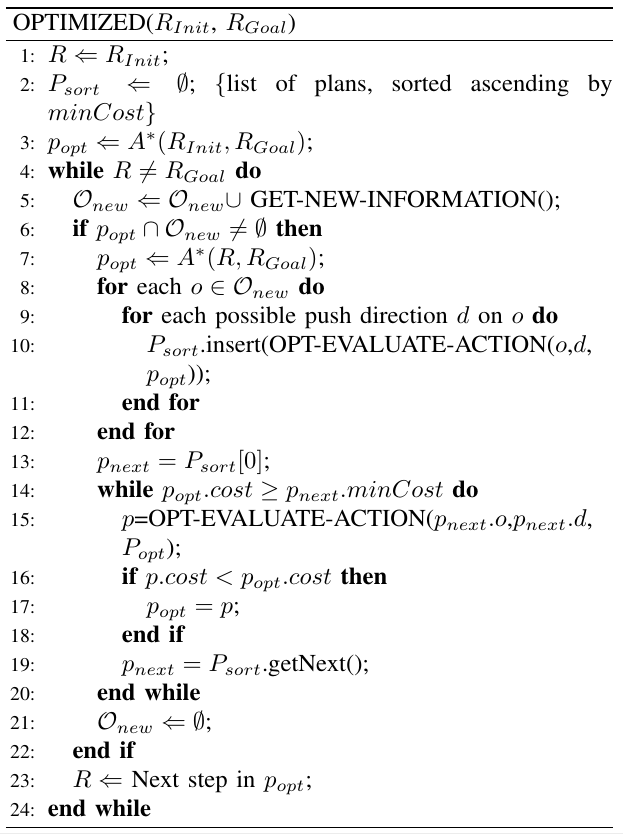
\includegraphics[width=\linewidth]{Figures/Wu_Original_Algorithm/algo3.png}
  \caption{Main loop}
  \label{fig:Wu_Original_Algorithm-algo3}
\end{subfigure}%
\begin{subfigure}{.5\textwidth}
  \centering
  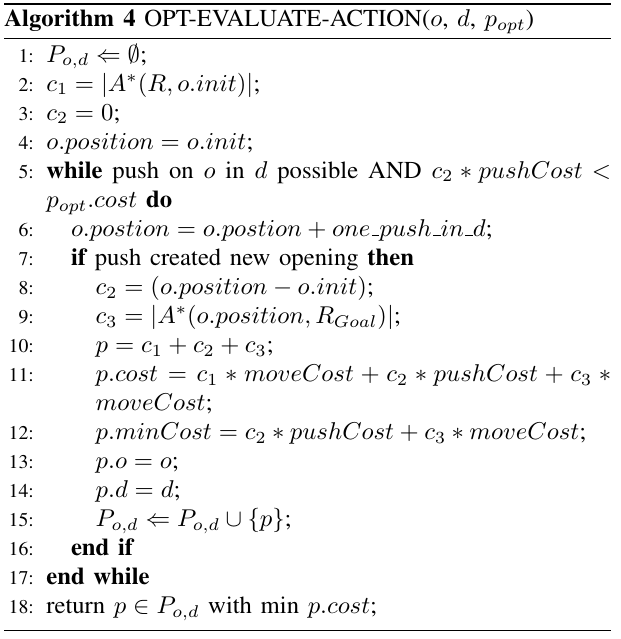
\includegraphics[width=\linewidth]{Figures/Wu_Original_Algorithm/algo4.png}
  \caption{Subroutine}
  \label{fig:Wu_Original_Algorithm-algo4}
\end{subfigure}
\caption{Optimized Algorithm as published by Wu et. al. in \parencite{wu_navigation_2010}}
\label{fig:Wu_Original_Algorithm-optimized}
\end{figure}

\section{Removing ambiguity}

\paragraph{A word on notations} The presented algorithms' pseudocode originally had some typos and mathematical incongruities like storing costs and paths in the same variable, confusing the reading. These mistakes have been fixed and for easier understanding, we will admit the following notations :

\begin{itemize}
  \item Paths (also called plans) will be noted with a lowercase $p$. Lists or sets of paths will be noted with an uppercase $P$.
  \item Paths are ordered sets of "steps", which are in fact 2D position vectors.
  \item Calling the A* or D*Lite algorithms returns A PATH if one is found, or null if none.
  \item Components of a path are subsets of consecutive "steps" (therefore, paths themselves) and are noted with a lowercase $c$.
  \item The norm of a path (written $|p|$) corresponds to the sum of the euclidean distances between consecutive steps, and $+\infty$ if the path is null.
  \item $moveCost$ and $pushCost$ are constants without dimension.
\end{itemize}

\paragraph{Note on Get-New-Information}\label{get-new-information_note} It is not explicit how this method works. It probaly fetches the new objects list from the robot's internal map, which would continuously be updated in another execution thread. Given that in our own hypothesis, we "know" that a movable obstacle

\paragraph{Note on Resetting the Current plan}\label{reset_plan_note} Reset the current plan from current robot position as the path that avoids all known objects.

\paragraph{Note on Re-evaluation}\label{re-evaluation_note} The way the pseudo-code is written, even new obstacles that have just been evaluated might be reevaluated, since they have been inserted into the $P_{sort}$ list right before. Consequently, we should add a condition $p_{next}.o \notin \mathcal{O}_{new}$ to execute the re-evaluation to optimize the algorithm further.

\paragraph{Note on bounding}\label{bound_note} Push until blocked (if the robot cannot get access to the grasping point required to move the object in a given direction or if there is a known obstacles that is going to enter in collision with the currently pushed obstacle, pushing must also be considered impossible) or pushing the object becomes more costly than avoiding the obstacle altogether. This is not a tight bound.

\paragraph{Note on Opening Detection}\label{opening_detection_note} It is not worth computing c2 and c3 if there is no new opening. Opening detection is not adressed in this paper and the method used is not explicit. The technical paper of Levihn and Stilman : "Efficient Opening Detection" (2011) says that : \textit{"The algorithm did not rely on search but simply observed the amount of adjacent free spaces on corners of the manipulated obstacle. While efficient, this algorithm is only applicable for world configurations populated with simple rectangular shaped static and movable obstacles. This is not realistic."}.

\paragraph{Note on the placement of the computation of $c2$}\label{c2_computation_note} $c2$ is only modified for each push \textbf{that creates a new opening} (as $c2$ is not defined if there is none ?). So if, for example, pushing 4 times an obstacle would result in overlapping the bound without creating an opening, the robot would still continue to simulate extra pushes until they are no longer possible (for example after 4 extra times) : given that detecting openings might be computationally expensive, \textbf{it would be better to exchange lines 35 and 36}, or at least, use a tighter bound that doesn't depend on $c2$.

\paragraph{Note on cost computation}\label{cost_computation_note} The formulation here is unclear, as it is not said how multiplying a trajectory by a constant creates a decimal number cost. A decent guess would be that we are in fact multiplying the distance traveled on each path by a constant which could be equivalent to a constant force to apply for accomplishing the action of moving or pushing, which would result in an energy ($distance*force=energy$).

\begin{algorithm}[H]

  \caption{Optimized algorithm for NAMO in unknown environments of Wu et. al. (2010), commented}

  \label{alg:namoue}

  \begin{algorithmic}[1]

      \Procedure{OPTIMIZED}{$R_{init}$, $R_{goal}$}

        \State $R \gets R_{init}$ \Comment{Current robot position initialization.}

        \State $P_{sort} \gets \emptyset$ \Comment{List of plans, ascendingly sorted by $minCost$.}

        \State $p_{opt} \gets A$*$(R_{init}, R_{goal})$ \Comment{Current plan initialized as simple A* path from init to goal.}

        \State $p_{opt}.cost \gets |p_{opt}| * moveCost$ \Comment{Added line for mathematical coherence.}

        \While{$R \neq R_{goal}$} \Comment{Stop only when goal is reached.}

          \State $\mathcal{O}_{new} \gets \mathcal{O}_{new} \bigcup$ GET-NEW-INFORMATION() \Comment{\nameref{get-new-information_note}}

          \If{$p_{opt} \bigcap \mathcal{O}_{new} \neq \emptyset$} \Comment{Recompute when new obstacles invalidate the current plan.}

            \State $p_{opt} \gets A$*($R$, $R_{goal}$) \Comment{\nameref{reset_plan_note}}
            \State $p_{opt}.cost \gets |p_{opt}| * moveCost$ \Comment{Added line for mathematical coherence.}

            \For{each $o \in \mathcal{O}_{new}$} \Comment{All new obstacles are evaluated for any displacements.}
              \For{each possible push direction $d$ on $o$}
                \State $P_{sort}$.insert(OPT-EVALUATE-ACTION($o$,$d$,$p_{opt}$))
              \EndFor
            \EndFor

            \State $p_{next} \gets P_{sort}[0]$ \Comment{Re-evaluate (older or not) plans that appear promising.}
            \While{$p_{opt}.cost \geq p_{next}.minCost$} \Comment{Loop until $p_{next}$ couldn't be better than $p_{opt}$.}
              \State $p \gets$ OPT-EVALUATE-ACTION($p_{next}.o, p_{next}.d, p_{opt}$) \Comment{\nameref{re-evaluation_note}}
              \If{$p.cost \leq p_{opt}.cost$}
                \State $p_{opt} \gets p$
              \EndIf
              \State $p_{next} \gets P_{sort}$.getNext()
            \EndWhile

            \State $\mathcal{O}_{new} \gets \emptyset$ \Comment{Reset so that only new objects are considered in the double-for loop.}

          \EndIf

          \State $R \gets$ Next step in $p_{opt}$ \Comment{\textbf{The robot's pose and what it perceives only change here.}}

        \EndWhile

    \EndProcedure

    \\

    \Procedure{OPT-EVALUATE-ACTION}{$o$, $d$, $p_{opt}$}

    \State $P_{o,d} \gets \emptyset$ \Comment{Unordered list for remembering a plan for each new opening.}
    \State $c_{1} \gets A$*$(R, o.init)$ \Comment{Path for reaching the contact point for pushing in $d$.}
    \State $c_{2} \gets \emptyset$ \Comment{Current path for moving $o$ in $d$}
    \State $o.position \gets o.init$ \Comment{$o.position$ and $o.init$ are both position vectors.}

    \While{push on $o$ in $d$ possible AND $|c_{2}| * pushCost \leq p_{opt}.cost$} \Comment{\nameref{bound_note}}
      \State $o.position \gets o.position + one\_push\_in\_d$ \Comment{Discrete pushes \textbf{only} in direction d.}
      \If{push created new opening} \Comment{\nameref{opening_detection_note}}
        \State $c_{2} \gets \{o.init, o.position\}$ \Comment{\nameref{c2_computation_note}}
        \State $c_{3} \gets A$*$(o.position, R_{goal})$ \Comment{Path from moved $o$ to the goal.}
        \State $p \gets c_{1} + c_{2} + c_{3}$ \Comment{Complete new path.}
        \State $p.cost \gets (|c_{1}| + |c_{3}|) * moveCost + |c_{2}| * pushCost$ \Comment{\nameref{cost_computation_note}}
        \State $p.minCost \gets |c_{2}| * pushCost + |c_{3}| * moveCost$ \Comment{Underestimated cost for the plan.}
        \State $p.o \gets o$ \Comment{A plan only implies one obstacle $o$,...}
        \State $p.d \gets d$ \Comment{... and a set of pushes in a single direction $d$.}
        \State $P_{o,d} \gets P_{o,d} \bigcup \{p\}$
      \EndIf
    \EndWhile

    \State return $p \in P_{o,d}$ with minimal $p.cost$ \Comment{Only return best plan.}

    \EndProcedure

  \end{algorithmic}

\end{algorithm}


\clearpage

\section{Pseudocode expression of Levihn's recommendations}

\subsection*{General notes}

\paragraph{Note on the use of highlighting}\label{highlight_note} \hlgreen{Green} highlights are for lines of the OPTIMIZED procedure that were \textbf{NOT} affected by the use of minCostL and euclideanCostL. \hlcyan{Blue} highlights are for lines of the OPT-EVALUATE-ACTION procedure that were \textbf{NOT} affected by the use $C_{est}$.

\subsection*{Notes on the improved obstacle evaluation}

\paragraph{Note on the computation of $c1$}\label{c1_computation_note} Computation for $c1$ (path component from robot position to object) is done only once for the object as the robot can just grasp any grasping point of the object, according to what Levihn allows (behaviour deducted from the \href{https://www.youtube.com/watch?v=3AvfPVzBb-s}{video}). This would not be possible if only push actions were considered, or the robot had to take holonomic or friction constraints into account.

\paragraph{Note on the computation of $C_{Est}$}\label{cest_computation_note} $C_{M}$ is a constant for the cost of the manipulation equivalent to the $pushCost$ in Wu's paper.

\paragraph{Note}\label{second_opening_detection_note} The method for detecting openings is explained in section \ref{eod_section} \nameref{eod_section}.

\subsection*{Notes on the improved estimation of candidate objects for evaluation}

\paragraph{Note on $euclideanCostL$}\label{euclideanCostL_note} Ordered list of tuples \{obstacle, $c_{3_{(Est)}}$\} ascendingly sorted by estimated euclidean cost assuming completely free space $c_{3_{(Est)}}$.

\paragraph{Note on $minCostL$}\label{minCostL_note} Ordered list of tuples \{obstacle, minCost\} ordered by minCost.

\paragraph{Note on free space creation}\label{free_space_note} Levihn's quote : \textit{"Second, as the algorithm does not acknowledge the fact that free-space can be created during the execution (e.g. by moving objects), which can lower c2 or c3 for some objects, this optimization steps sacrifices local optimality."} . Thus we will consider that any successful manipulation of an object creates new free space (the place it occupied is freed).

\paragraph{Note on the underestimate guarantee of minCostL}\label{underestimate_note} The lists $minCostL$ and $euclideanCostL$ contain underestimates of the cost of moving an object. For $euclideanCostL$, this is guaranteed by the constant update of the $c_{3_{est}}$, which is, for remembrance, the estimated euclidean cost between the current robot and object positions, assuming completely free space. For $minCostL$, the guarantee is not as trivial since its elements are only guaranteed to be underestimates, citing Levihn : \textit{"if no new free-space has been created since the entries were generated : If free-space is created, for example by the robot moving objects, it is possible that entries in minCostL are overestimating the plan cost for specific objects as the newly generated free-space might give rise to simpler manipulation plans for the objects."}. According to Levihn's work, we empty $minCostL$ as soon as new free space is detected so that its elements cannot become overestimates in any case. Concretely, detecting new free space will probably be done by simply detecting whether any object has moved or not.

\paragraph{Note on getting the list element and limit cases}\label{get_list_element_note} For the sake of readability in the pseudocode, if the list element that is asked for is out of bounds (empty list or reached end of list), the "[ ]" operator shall return a "fake" tuple with empty obstacle reference, and infinite cost : \{null, $+\infty$\}. This could easily be implented in code by either using a ternary operator (for example, "$minCostL[i_{m}].minCost$" would become "$minCostL[i_{m}] =$ null ? $+\infty : minCostL[i_{m}].minCost$") or implementing a custom array object with the wanted behaviour.

\paragraph{Note}\label{list_traversal_note} If the next entry from $minCostL$ or $euclideanCostL$ to be considered (the one with the lowest cost) is associated with a cost that is greater than the current optimal plan, it is not worth trying to evaluate any more options, and therefore the loop must end.

\paragraph{Note on the priority}\label{minCostL_priority_note}If the current lowest cost entry is minCostL, evaluate the associated obstacle.

\paragraph{Postponing}\label{postponing_note} If $i_{e}$ points to a lower cost, we only evaluate the associated object if $minCostL$ doesn't already contain an evaluation for it, therefore, it means there is tighter bound for the cost of moving the object, and evaluation can be postponed.

\paragraph{Note on OPT-EVALUATE-ACTION's return values}\label{opt_return_note} If no path has been found, $P_{o,m} = \emptyset$, then $p$ is affected with the "null" value.

\begin{algorithm}[H]

  \caption{Optimized algorithm for NAMO in unknown environments of Wu et. al. adapted according to M.Levihn et. al.'s (2014) recommandations. \nameref{highlight_note}}

  \label{alg:namoue_augmented}

  \begin{algorithmic}[1]

      \Procedure{OPTIMIZED}{$R_{init}$, $R_{goal}$}

        \State \hlgreen{$R \gets R_{init}$}
        \State $euclideanCostL \gets \emptyset$ \Comment{\nameref{euclideanCostL_note}}
        \State $minCostL \gets \emptyset$ \Comment{\nameref{minCostL_note}}
        \State $p_{opt}.path \gets D$*Lite($R_{init}$, $R_{goal}$, $empty\_occupation\_grid$) \Comment{Calls to A* replaced by D*Lite.}

        \State \hlgreen{$p_{opt}.cost \gets |p_{opt}| * moveCost$}

        \While{\hlgreen{$R \neq R_{goal}$}}

        \State $G \gets $ GET-NEW-INFORMATION()

        \If{$G.freeSpaceCreated$} \Comment{\nameref{free_space_note}}
          \State $minCostL$.empty() \Comment{\nameref{underestimate_note}}
        \EndIf

        \State $\mathcal{O}_{new} \gets \mathcal{O}_{new} \bigcup G.$newObstacles()

          \If{\hlgreen{$p_{opt} \bigcap \mathcal{O}_{new} \neq \emptyset$}}

            \State $\mathcal{O} \gets \mathcal{O} \bigcup \mathcal{O}_{new}$

            \For{each $o \in \mathcal{O}$}
              \State $euclideanCostL$.insertOrUpdate$(\{o, |o.center - R.goal|\})$
            \EndFor

            \State $p_{opt}.path \gets D$*Lite($R$, $R_{goal}$, $G$)
            \State \hlgreen{$p_{opt}.cost \gets |p_{opt}| * moveCost$}

            \State $i_{e}, i_{m} \gets 0 , 0$ \Comment{\nameref{get_list_element_note}}

            \While{$\min(minCostL[i_{m}].minCost, euclideanCostL[i_{e}].c_{3_{est}}) < p_{opt}.cost$}
              \Comment{\nameref{list_traversal_note}}
              \If{$minCostL[i_{m}].minCost < euclideanCostL[i_{e}].c_{3_{est}}$} \Comment{\nameref{minCostL_priority_note}}
                \State $p \gets$ OPT-EVALUATE-ACTION($minCostL[i_{m}].obstacle$, $p_{opt}$, $G$, $R$, $R_{goal}$)
                \If{$p \neq$ null} \Comment{Check if a new path has been found.}
                  \State $minCostL.$insertOrUpdate$(\{minCostL[i_{m}].obstacle, p.minCost\})$
                  \State $i_{m} \gets i_{m} + 1$ \Comment{Point to $minCostL$'s next entry.}
                  \If{$p.cost < p_{opt}.cost$} \Comment{Replace current optimal plan if $p$ is better.}
                    \State $p_{opt} \gets p$
                  \EndIf
                \EndIf
              \Else
                \If{$minCostL$.contains($euclideanCostL[i_{e}].obstacle) = false$}
                \Comment{\nameref{postponing_note}}
                  \State $p \gets$ OPT-EVALUATE-ACTION($euclideanCostL[i_{e}].obstacle$, $p_{opt}$, $G$, $R$, $R_{goal}$)
                  \If{$p \neq$ null}
                    \State $minCostL.$insertOrUpdate$(\{euclideanCostL[i_{e}].obstacle, p.minCost\})$
                    \State $i_{m} \gets i_{m} + 1$
                    \If{$p.cost < p_{opt}.cost$}
                      \State $p_{opt} \gets p$
                    \EndIf
                  \EndIf
                \EndIf
              \EndIf
              \State $i_{e} \gets i_{e} + 1$ \Comment{The pointer $i_{e}$ is always incremented.}
            \EndWhile
            \State \hlgreen{$\mathcal{O}_{new} \gets \emptyset$}
          \EndIf
          \State \hlgreen{$R \gets$ Next step in $p_{opt}$} \Comment{If $p_{opt} =$ null, stop the robot and signal that it is blocked.}
        \EndWhile
    \EndProcedure

    \algstore{namoue_augmented}

  \end{algorithmic}
\end{algorithm}

\begin{algorithm}[H]
  \begin{algorithmic}[1]
    \algrestore{namoue_augmented}

    \Procedure{OPT-EVALUATE-ACTION}{$o$, $p_{opt}$, $G$, $R$, $R_{goal}$}

      \State $P_{o,m}$ $\gets \emptyset$
      \State $c_{1} \gets D$*Lite$(R, o.init, $G$)$ \Comment{\nameref{c1_computation_note}}
      \State $BA \gets null$ \Comment{Remember blocking areas for more efficient opening detection.}

      \For{each possible manipulation $m$ on $o$}

        \State $seq \gets 1$ \Comment{Current depth of the search, initialized to 1.}

        \State $c_{3_{(Est)}} \gets \{o.position, R_{goal}\}$ \Comment{Straight line between grasping point and goal.}

        \State $C_{est} \gets |c_{1}| + seq * C_{M} + |c_{3_{(Est)}}|$ \Comment{\nameref{cest_computation_note}}

        \State $oSimPosition \gets o.init + next\_manipulation\_step$

        \While{manipulation on $o$ possible AND $C_{est}$ $ \leq p_{opt}.cost$}

          \If{CHECK-NEW-OPENING($G$, $o$, $next\_manipulation\_step$, $BA$)} \Comment{\nameref{second_opening_detection_note}}
            \State \hlcyan{$c_{2} \gets \{o.init, oSimPosition\}$} \Comment{Supposing we still only push or pull in one direction.}
            \State $c_{3} \gets D$*Lite($oSimPosition$, $R_{goal}$, $G$)
            \State \hlcyan{$p.path \gets c_{1} + c_{2} + c_{3}$}
            \State $p.cost \gets (|c_{1}| + |c_{3}|) * moveCost + |c_{2}| * C_{M}$
            \State $p.minCost \gets |c_{2}| * C_{M} + |c_{3}| * moveCost$
            \State \hlcyan{$p.o \gets o$}
            \State $p.m \gets m$
            \State $P_{o,m} \gets P_{o,m} \bigcup \{p\}$
          \EndIf

          \State $oSimPosition \gets oSimPosition + next\_manipulation\_step$

          \State $seq \gets seq + 1$ \Comment{Increment depth of search for next loop.}

          \State $c_{3_{(Est)}} \gets \{oSimPosition, R_{goal}\}$

          \State $C_{est} \gets |c_{1}| + seq * C_{M} + |c_{3_{(Est)}}|$ \Comment{Update $C_{est}$ for next loop}

        \EndWhile

      \EndFor

    \State return $p \in P_{o,m}$ with minimal $p.cost$ \Comment{\nameref{opt_return_note}}

    \EndProcedure

  \end{algorithmic}
\end{algorithm}


\section{Discussion on the hypotheses of the original algorithms according to test with the Pepper robot}
